\documentclass[report.tex]{subfiles}
\begin{document}
\subsection{Methodology}
\label{sec:lab2 methodology}
This section is divided in three parts:
\begin{itemize}
    \item Introduction to S-parameter simulation
    \item Unmatched NPN transistor
    \item Impedance matched NPN transistor
\end{itemize}
%The first part will give a basic introduction on how S-parameter simulation is performed in ADS.
%
%The second part will focus on how impedance matching affects a system at high frequency and why it is important to have matching networks.
%
%The last part will go into detail on how impedance matching can be achieved in ADS.

\subsubsection{Introduction to S-parameter simulation}
Three basic components - resistor, inductor, capacitor - are simulated in a network with an characteristic impedance of $50~\Omega$. Figure~\ref{fig:problem 1 circuit} show the simulation setup for a $50~\Omega$ resistor. The other two basic component were simulated using the same setup, substituting the resistor with a $2~\text{nH}$ inductor or $3~\text{pF}$ capacitor.

Results of the simulations is found in chapter \ref{sec:lab2_results}.

\begin{figure}[h]
    \centering
    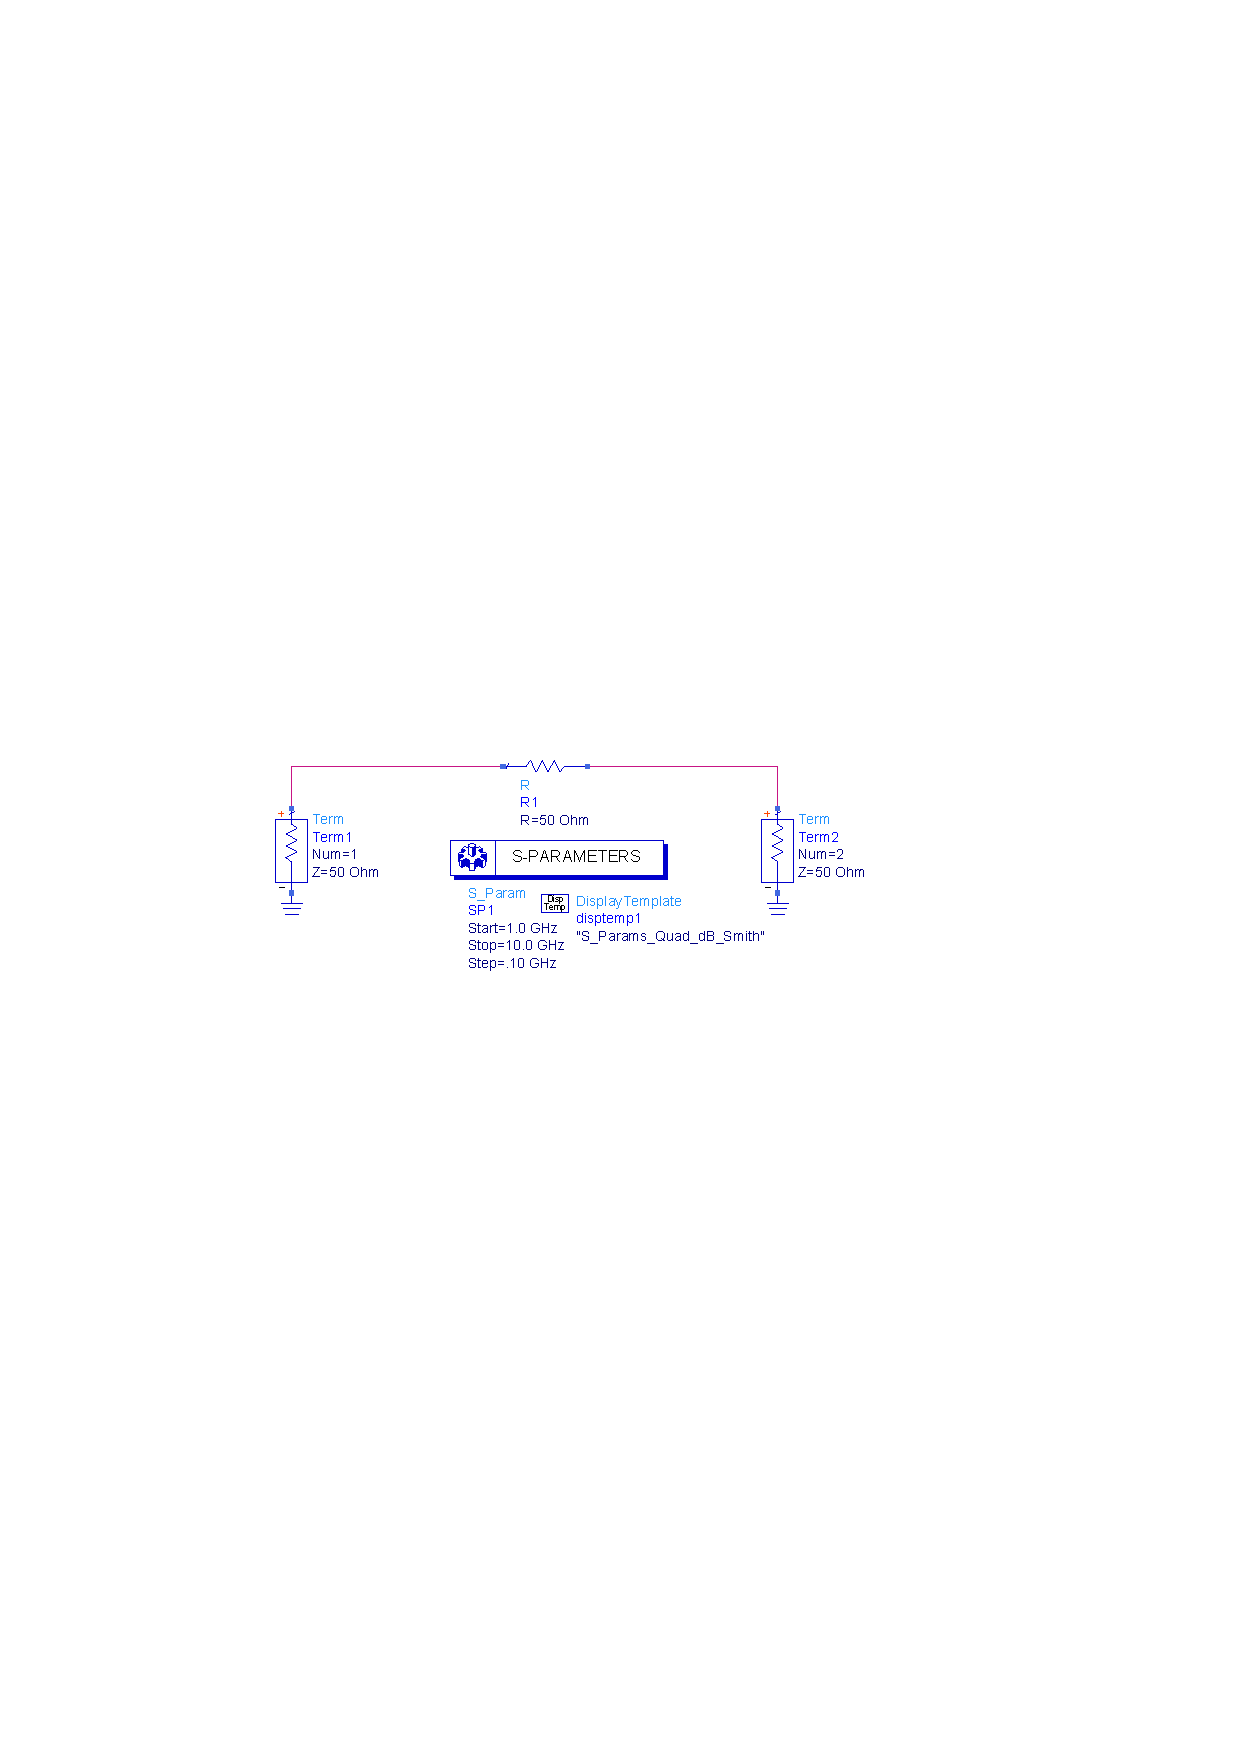
\includegraphics[width=\textwidth]{problem_1_circuit}
    \caption{Simulation setup}
    \label{fig:problem 1 circuit}
\end{figure}

\subsubsection{Unmatched NPN transistor}
To simulate an NPN transistor that is more true-to-life, several parasitic inductances and capacitances are introduced. The complete simulation setup for a unmatched NPN transistor network connected to a $50~\Omega$ source and load is shown in fig.~\ref{fig:problem 2A circuit}.

The simulation result for fig.~\ref{fig:problem 2A circuit} is found in chapter \ref{sec:lab2_results}.

\begin{figure}[h]
    \centering
    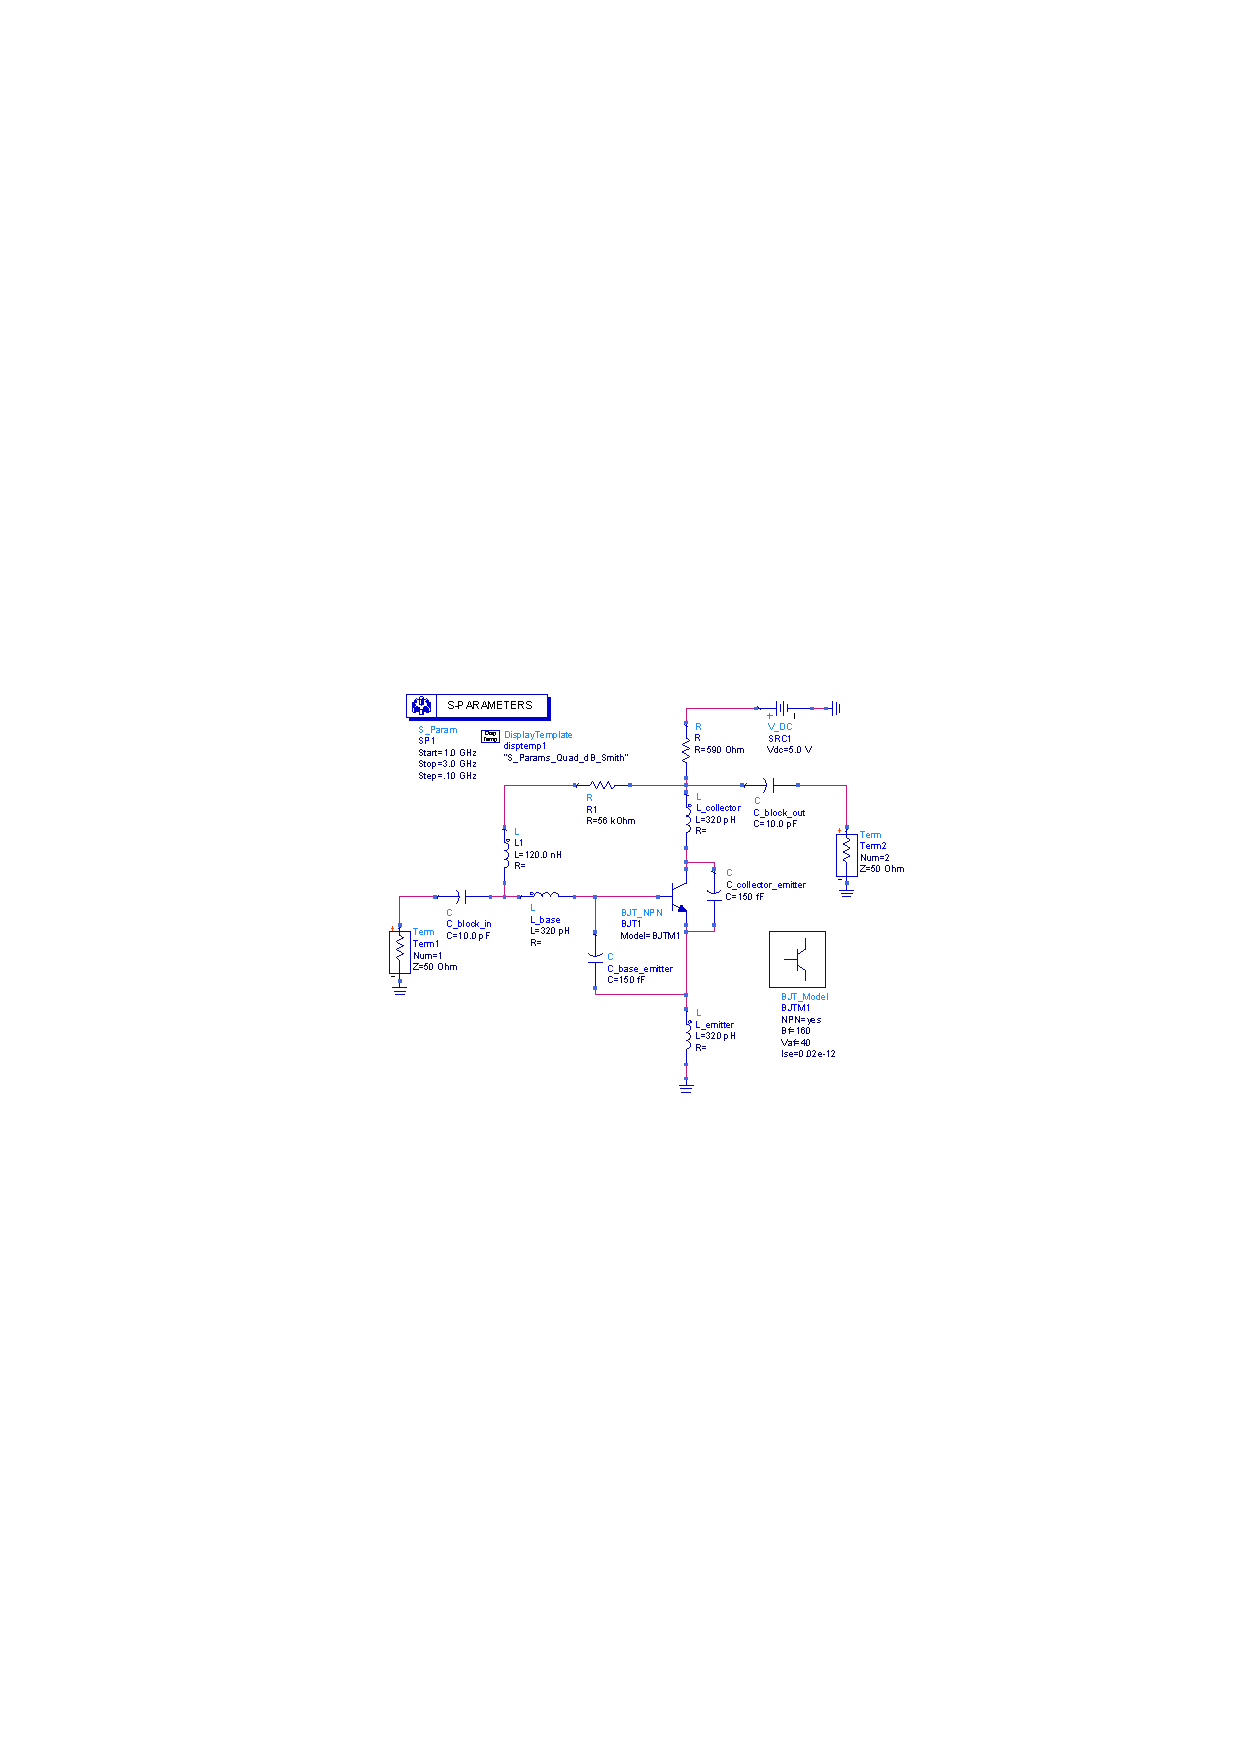
\includegraphics[width=\textwidth]{problem_2A_circuit}
    \caption{Unmatched NPN transistor network}
    \label{fig:problem 2A circuit}
\end{figure}

\subsubsection{Impedance matched NPN transistor}
By using the DesignGuide (\emph{Filter/Smith Chart}) in ADS and applying the same graphical method as described in chapter~\ref{seq:lab2 background}, both an input and output matching network can be derived.

The parameters derived from DesignGuide can be even further tuned by using the ADS tool ``tune". With the ``tune" utility, all relevant parameter can be put together and then individually altered, and the effect of the adjustments are instantly reflected in the simulation results.

The final impedance matched schematic is shown in fig.~\ref{fig:problem 2C circuit} and the simulation results are summarized in chapter \ref{sec:lab2_results}.

\begin{figure}[h]
    \centering
    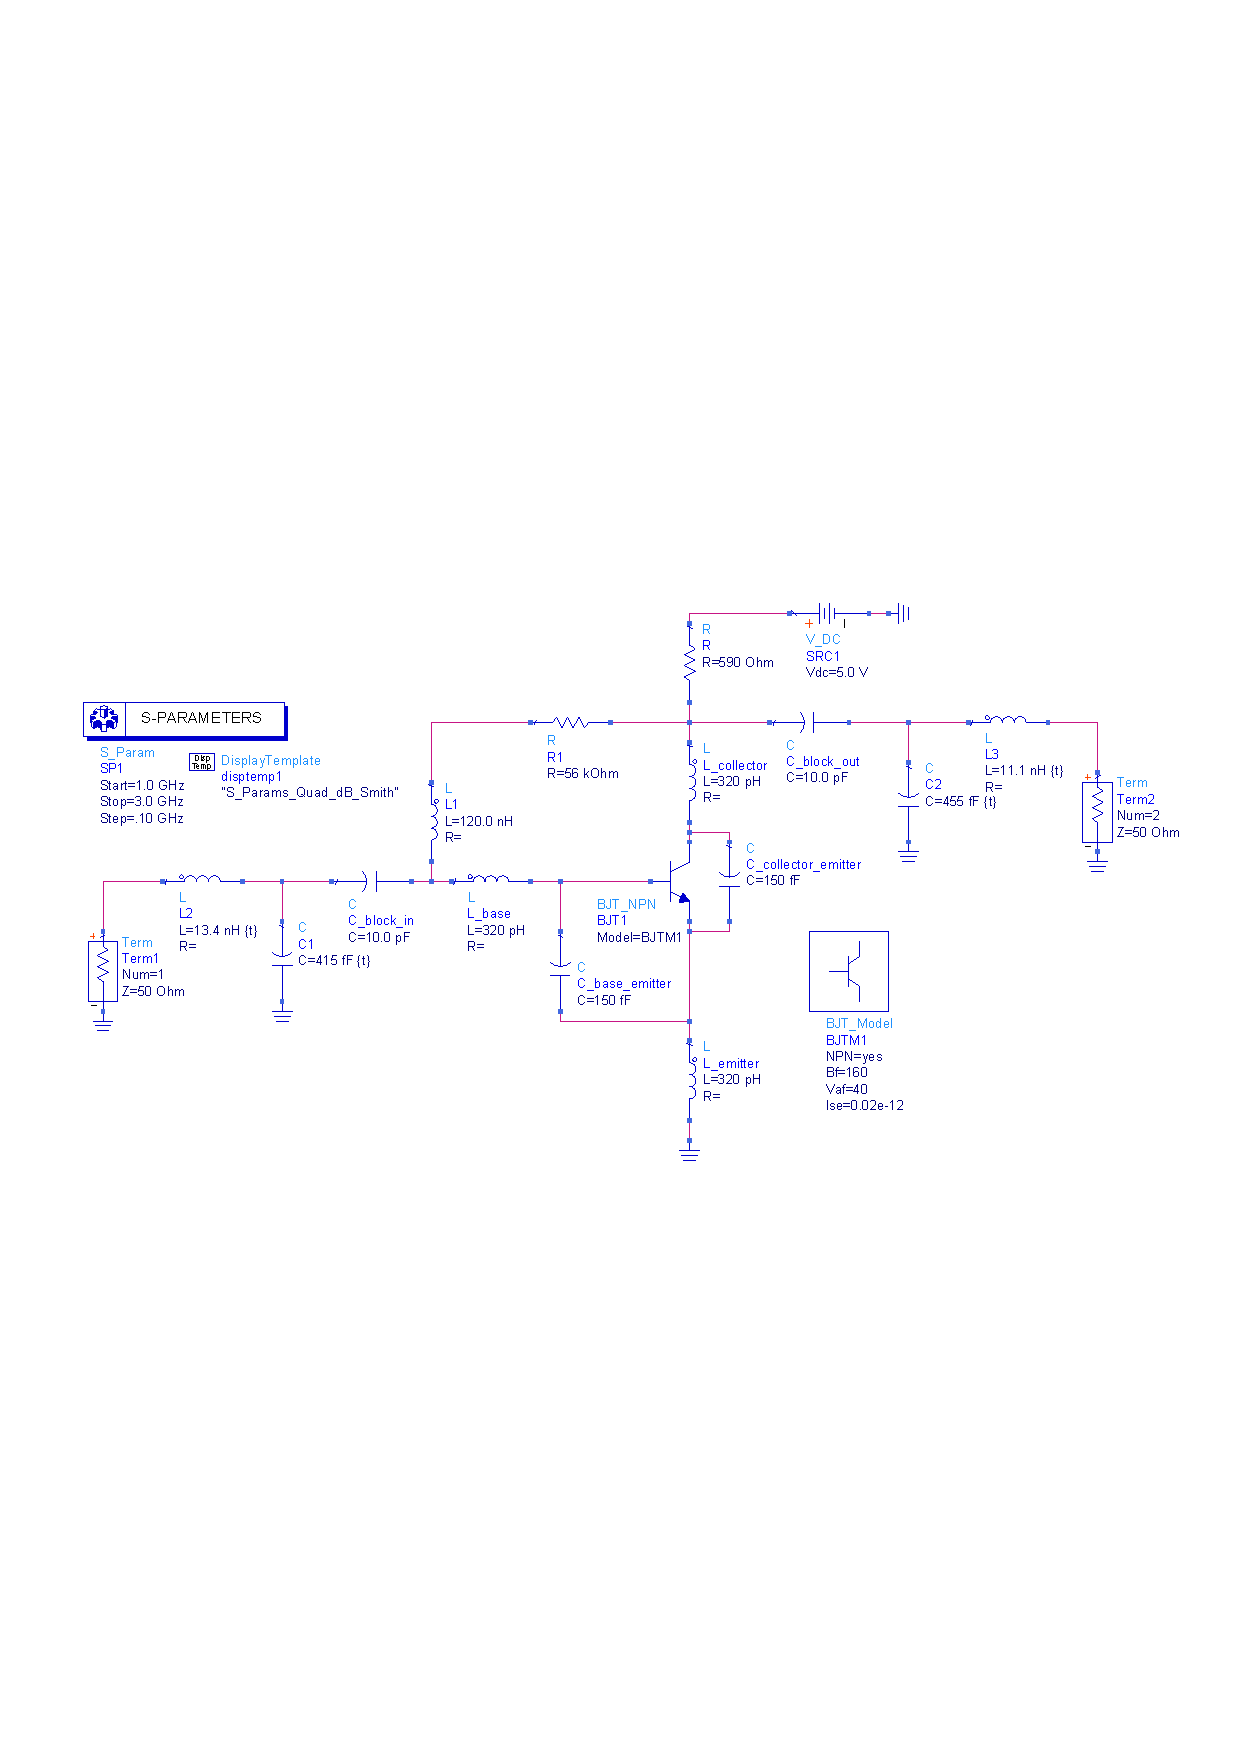
\includegraphics[width=\textwidth]{problem_2C_circuit}
    \caption{Impedance matched NPN transistor network}
    \label{fig:problem 2C circuit}
\end{figure}

\end{document}